% !TeX spellcheck = pl_PL
%%%%%%%%%%%%%%%%%%%%%%%%%%%%%%%%%%%%%%%%%%%
%                                        %
% Szablon pracy dyplomowej inzynierskiej %
% zgodny  z aktualnymi  przepisami  SZJK %
%                                        %
%%%%%%%%%%%%%%%%%%%%%%%%%%%%%%%%%%%%%%%%%%
%                                        %
%  (c) Krzysztof Simiński, 2018-2023     %
%                                        %
%%%%%%%%%%%%%%%%%%%%%%%%%%%%%%%%%%%%%%%%%%
%                                        %
% Najnowsza wersja szablonów jest        %
% podstępna pod adresem                  %
% github.com/ksiminski/polsl-aei-theses  %
%                                        %
%%%%%%%%%%%%%%%%%%%%%%%%%%%%%%%%%%%%%%%%%%
%
%
% Projekt LaTeXowy zapewnia odpowiednie formatowanie pracy,
% zgodnie z wymaganiami Systemu zapewniania jakości kształcenia.
% Proszę nie zmieniać ustawień formatowania (np. fontu,
% marginesów, wytłuszczeń, kursywy itd. ).
%
% Projekt można kompilować na kilka sposobów.
%
% 1. kompilacja pdfLaTeX
%
% pdflatex main
% bibtex   main
% pdflatex main
% pdflatex main
%
%
% 2. kompilacja XeLaTeX
%
% Kompilatacja przy użyciu XeLaTeXa różni się tym, że na stronie
% tytułowej używany jest font Calibri. Wymaga to jego uprzedniego
% zainstalowania.
%
% xelatex main
% bibtex  main
% xelatex main
% xelatex main
%
%
%%%%%%%%%%%%%%%%%%%%%%%%%%%%%%%%%%%%%%%%%%%%%%%%%%%%%
% W przypadku pytań, uwag, proszę pisać na adres:   %
%      krzysztof.siminski(małpa)polsl.pl            %
%%%%%%%%%%%%%%%%%%%%%%%%%%%%%%%%%%%%%%%%%%%%%%%%%%%%%
%
% Chcemy ulepszać szablony LaTeXowe prac dyplomowych.
% Wypełniając ankietę spod poniższego adresu pomogą
% Państwo nam to zrobić. Ankieta jest całkowicie
% anonimowa. Dziękujemy!


% https://docs.google.com/forms/d/e/1FAIpQLScyllVxNKzKFHfILDfdbwC-jvT8YL0RSTFs-s27UGw9CKn-fQ/viewform?usp=sf_link
%
%%%%%%%%%%%%%%%%%%%%%%%%%%%%%%%%%%%%%%%%%%%%%%%%%%%%%%%%%%%%%%%%%%%%%%%%%

%%%%%%%%%%%%%%%%%%%%%%%%%%%%%%%%%%%%%%%%%%%%%%%
%                                             %
% PERSONALIZACJA PRACY – DANE PRACY           %
%                                             %
%%%%%%%%%%%%%%%%%%%%%%%%%%%%%%%%%%%%%%%%%%%%%%%

% Proszę wpisać swoje dane w poniższych definicjach.

% TODO
% dane autora
\newcommand{\FirstNameAuthor}{Jagoda}
\newcommand{\SurnameAuthor}{Więcek}
\newcommand{\IdAuthor}{300503}   % numer albumu  (bez $\langle$ i $\rangle$)

% drugi autor:
%\newcommand{\FirstNameCoauthor}{Imię}   % Jeżeli jest drugi autor, to tutaj należy podać imię.
%\newcommand{\SurnameCoauthor}{Nazwisko} % Jeżeli jest drugi autor, to tutaj należy podać nazwisko.
%\newcommand{\IdCoauthor}{$\langle$wpisać właściwy$\rangle$}  % numer albumu drugiego autora (bez $\langle$ i $\rangle$)
% Gdy nie ma drugiego autora, należy zostawić poniższe definicje puste, jak poniżej. Gdy jest drugi autor, należy zakomentować te linie.
\newcommand{\FirstNameCoauthor}{} % Jeżeli praca ma tylko jednego autora, to dane drugiego autora zostają puste.
\newcommand{\SurnameCoauthor}{}   % Jeżeli praca ma tylko jednego autora, to dane drugiego autora zostają puste.
\newcommand{\IdCoauthor}{}  % Jeżeli praca ma tylko jednego autora, to dane drugiego autora zostają puste.
%%%%%%%%%%

\newcommand{\Supervisor}{Dr inż. Ewa Lach}     % dane promotora (bez $\langle$ i $\rangle$)
\newcommand{\Title}{Gra planszowa 2.5D z uczeniem maszynowym komputerowych graczy}           % tytuł pracy po polsku
\newcommand{\TitleAlt}{2.5D board game with machine learning for computer players}                     % thesis title in English
\newcommand{\Program}{Informatyka}            % kierunek studiów  (bez $\langle$ i $\rangle$)
\newcommand{\Specialisation}{Grafika Komputerowa i Oprogramowanie}     % specjalność  (bez $\langle$ i $\rangle$)
\newcommand{\Departament}{Grafiki, Wizji Komputerowej i Systemów Cyfrowych}        % katedra promotora  (bez $\langle$ i $\rangle$)


% ... w przeciwnym razie proszę zostawić puste miejsce jak poniżej:
%\newcommand{\Consultant}{} % brak promotowa pomocniczego / opiekuna

% koniec fragmentu do modyfikacji
%%%%%%%%%%%%%%%%%%%%%%%%%%%%%%%%%%%%%%%%%%


%%%%%%%%%%%%%%%%%%%%%%%%%%%%%%%%%%%%%%%%%%%%%%%
%                                             %
% KONIEC PERSONALIZACJI PRACY                 %
%                                             %
%%%%%%%%%%%%%%%%%%%%%%%%%%%%%%%%%%%%%%%%%%%%%%%

%%%%%%%%%%%%%%%%%%%%%%%%%%%%%%%%%%%%%%%%


%%%%%%%%%%%%%%%%%%%%%%%%%%%%%%%%%%%%%%%%%%%%%%%
%                                             %
% PROSZĘ NIE MODYFIKOWAĆ PONIŻSZYCH USTAWIEŃ! %
%                                             %
%%%%%%%%%%%%%%%%%%%%%%%%%%%%%%%%%%%%%%%%%%%%%%%



\documentclass[a4paper,twoside,12pt]{book}
\usepackage[utf8]{inputenc}                                      
\usepackage[T1]{fontenc}  
\usepackage{amsmath,amsfonts,amssymb,amsthm}
\usepackage[british,polish]{babel} 
\usepackage{indentfirst}
\usepackage{xurl}
\usepackage{xstring}
\usepackage{ifthen}

\usepackage{placeins}

\usepackage{ifxetex}

\ifxetex
\usepackage{fontspec}
\defaultfontfeatures{Mapping=tex—text} % to support TeX conventions like ``——-''
\usepackage{xunicode} % Unicode support for LaTeX character names (accents, European chars, etc)
\usepackage{xltxtra} % Extra customizations for XeLaTeX
\else
\usepackage{lmodern}
\fi



\usepackage[margin=2.5cm]{geometry}
\usepackage{graphicx} 
%\usepackage{hyperref}
\usepackage{booktabs}
\usepackage{tikz}
\usepackage{pgfplots}
\usepackage{mathtools}
\usepackage{geometry}
\usepackage{subcaption}   % subfigures
\usepackage[page]{appendix} % toc,
\renewcommand{\appendixtocname}{Dodatki}
\renewcommand{\appendixpagename}{Dodatki}
\renewcommand{\appendixname}{Dodatek}

\usepackage{csquotes}
\usepackage[natbib=true,backend=bibtex,maxbibnames=99]{biblatex}  % kompilacja bibliografii BibTeXem
%\usepackage[natbib=true,backend=biber,maxbibnames=99]{biblatex}  % kompilacja bibliografii Biberem
\bibliography{biblio}

\usepackage{ifmtarg}   % empty commands  

\usepackage{setspace}
\usepackage{float}
\onehalfspacing


\frenchspacing



%%%% TODO LIST GENERATOR %%%%%%%%%

\usepackage{color}
\definecolor{brickred}      {cmyk}{0   , 0.89, 0.94, 0.28}

\makeatletter \newcommand \kslistofremarks{\section*{Uwagi} \@starttoc{rks}}
\newcommand\l@uwagas[2]
{\par\noindent \textbf{#2:} %\parbox{10cm}
	{#1}\par} \makeatother


\newcommand{\ksremark}[1]{%
	{%\marginpar{\textdbend}
		{\color{brickred}{[#1]}}}%
	\addcontentsline{rks}{uwagas}{\protect{#1}}%
}

\newcommand{\comma}{\ksremark{przecinek}}
\newcommand{\nocomma}{\ksremark{bez przecinka}}
\newcommand{\styl}{\ksremark{styl}}
\newcommand{\ortografia}{\ksremark{ortografia}}
\newcommand{\fleksja}{\ksremark{fleksja}}
\newcommand{\pauza}{\ksremark{pauza `--', nie dywiz `-'}}
\newcommand{\kolokwializm}{\ksremark{kolokwializm}}
\newcommand{\cudzyslowy}{\ksremark{,,polskie cudzysłowy''}}

%%%%%%%%%%%%%% END OF TODO LIST GENERATOR %%%%%%%%%%%

\newcommand{\printCoauthor}{%		
	\StrLen{\FirstNameCoauthor}[\FNCoALen]
	\ifthenelse{\FNCoALen > 0}%
	{%
		{\large\bfseries\Coauthor\par}
		
		{\normalsize\bfseries \LeftId: \IdCoauthor\par}
	}%
	{}
} 

%%%%%%%%%%%%%%%%%%%%%
\newcommand{\autor}{%		
	\StrLen{\FirstNameCoauthor}[\FNCoALenXX]
	\ifthenelse{\FNCoALenXX > 0}%
	{\FirstNameAuthor\ \SurnameAuthor, \FirstNameCoauthor\ \SurnameCoauthor}%
	{\FirstNameAuthor\ \SurnameAuthor}%
}
%%%%%%%%%%%%%%%%%%%%%

\StrLen{\FirstNameCoauthor}[\FNCoALen]
\ifthenelse{\FNCoALen > 0}%
{%
	\author{\FirstNameAuthor\ \SurnameAuthor, \FirstNameCoauthor\ \SurnameCoauthor}
}%
{%
	\author{\FirstNameAuthor\ \SurnameAuthor}
}%

%%%%%%%%%%%% ZYWA PAGINA %%%%%%%%%%%%%%%
% brak kapitalizacji zywej paginy
\usepackage{fancyhdr}
\pagestyle{fancy}
\fancyhf{}
\fancyhead[LO]{\nouppercase{\it\rightmark}}
\fancyhead[RE]{\nouppercase{\it\leftmark}}
\fancyhead[LE,RO]{\it\thepage}


\fancypagestyle{tylkoNumeryStron}{%
	\fancyhf{} 
	\fancyhead[LE,RO]{\it\thepage}
}

\fancypagestyle{bezNumeracji}{%
	\fancyhf{} 
	\fancyhead[LE,RO]{}
}


\fancypagestyle{NumeryStronNazwyRozdzialow}{%
	\fancyhf{} 
	\fancyhead[LE]{\nouppercase{\autor}}
	\fancyhead[RO]{\nouppercase{\leftmark}} 
	\fancyfoot[CE, CO]{\thepage}
}


%%%%%%%%%%%%% OBCE WTRETY  
\newcommand{\obcy}[1]{\emph{#1}}
\newcommand{\english}[1]{{\selectlanguage{british}\obcy{#1}}}
%%%%%%%%%%%%%%%%%%%%%%%%%%%%%

% polskie oznaczenia funkcji matematycznych
\renewcommand{\tan}{\operatorname {tg}}
\renewcommand{\log}{\operatorname {lg}}

% jeszcze jakies drobiazgi

\newcounter{stronyPozaNumeracja}

%%%%%%%%%%%%%%%%%%%%%%%%%%% 
\newcommand{\printOpiekun}[1]{%		
	
	\StrLen{\Consultant}[\mystringlen]
	\ifthenelse{\mystringlen > 0}%
	{%
		{\large{\bfseries OPIEKUN, PROMOTOR POMOCNICZY}\par}
		
		{\large{\bfseries \Consultant}\par}
	}%
	{}
} 
%
%%%%%%%%%%%%%%%%%%%%%%%%%%%%%%%%%%%%%%%%%%%%%%

% Proszę nie modyfikować poniższych definicji!
\newcommand{\Author}{\FirstNameAuthor\ \MakeUppercase{\SurnameAuthor}} 
\newcommand{\Coauthor}{\FirstNameCoauthor\ \MakeUppercase{\SurnameCoauthor}}
\newcommand{\Type}{PROJEKT INŻYNIERSKI}
\newcommand{\Faculty}{Wydział Automatyki, Elektroniki i Informatyki} 
\newcommand{\Polsl}{Politechnika Śląska}
\newcommand{\Logo}{politechnika_sl_logo_bw_pion_pl.pdf}
\newcommand{\LeftId}{Nr albumu}
\newcommand{\LeftProgram}{Kierunek}
\newcommand{\LeftSpecialisation}{Specjalność}
\newcommand{\LeftSUPERVISOR}{PROWADZĄCY PRACĘ}
\newcommand{\LeftDEPARTMENT}{KATEDRA}
%%%%%%%%%%%%%%%%%%%%%%%%%%%%%%%%%%%%%%%%%%%%%%

%%%%%%%%%%%%%%%%%%%%%%%%%%%%%%%%%%%%%%%%%%%%%%%
%                                             %
% KONIEC USTAWIEŃ                             %
%                                             %
%%%%%%%%%%%%%%%%%%%%%%%%%%%%%%%%%%%%%%%%%%%%%%%




%%%%%%%%%%%%%%%%%%%%%%%%%%%%%%%%%%%%%%%%%%%%%%%
%                                             %
% MOJE PAKIETY, USTAWIENIA ITD                %
%                                             %
%%%%%%%%%%%%%%%%%%%%%%%%%%%%%%%%%%%%%%%%%%%%%%%

% Tutaj proszę umieszczać swoje pakiety, makra, ustawienia itd.



%%%%%%%%%%%%%%%%%%%%%%%%%%%%%%%%%%%%%%%%%%%%%%%%%%%%%%%%%%%%%%%%%%%%%
% listingi i fragmentu kodu źródłowego 
% pakiet: listings lub minted
% % % % % % % % % % % % % % % % % % % % % % % % % % % % % % % % % % % 

% biblioteka listings
\usepackage{listings}
\lstset{%
	morekeywords={string,exception,std,vector},% słowa kluczowe rozpoznawane przez pakiet listings
	language=C++,% C, Matlab, Python, SQL, TeX, XML, bash, ... – vide https://www.ctan.org/pkg/listings
	commentstyle=\textit,%
	identifierstyle=\textsf,%
	keywordstyle=\sffamily\bfseries, %\texttt, %
	%captionpos=b,%
	tabsize=3,%
	frame=lines,%
	numbers=left,%
	numberstyle=\tiny,%
	numbersep=5pt,%
	breaklines=true,%
	escapeinside={@*}{*@},%
}

% % % % % % % % % % % % % % % % % % % % % % % % % % % % % % % % % % % 
% pakiet minted
%\usepackage{minted}

% pakiet wymaga specjalnego kompilowania:
% pdflatex -shell-escape main.tex
% xelatex  -shell-escape main.tex

%\usepackage[chapter]{minted} % [section]
%%\usemintedstyle{bw}   % czarno-białe kody 
%
%\setminted % https://ctan.org/pkg/minted
%{
	%%fontsize=\normalsize,%\footnotesize,
	%%captionpos=b,%
	%tabsize=3,%
	%frame=lines,%
	%framesep=2mm,
	%numbers=left,%
	%numbersep=5pt,%
	%breaklines=true,%
	%escapeinside=@@,%
	%}

%%%%%%%%%%%%%%%%%%%%%%%%%%%%%%%%%%%%%%%%%%%%%%%%%%%%%%%%%%%%%%%%%%%%%



%%%%%%%%%%%%%%%%%%%%%%%%%%%%%%%%%%%%%%%%%%%%%%%
%                                             %
% KONIEC MOICH USTAWIEŃ                       %
%                                             %
%%%%%%%%%%%%%%%%%%%%%%%%%%%%%%%%%%%%%%%%%%%%%%%



%%%%%%%%%%%%%%%%%%%%%%%%%%%%%%%%%%%%%%%%


\begin{document}
	%\kslistofremarks
	
	\frontmatter
	
	%%%%%%%%%%%%%%%%%%%%%%%%%%%%%%%%%%%%%%%%%%%%%%%
	%                                             %
	% PROSZĘ NIE MODYFIKOWAĆ STRONY TYTUŁOWEJ!    %
	%                                             %
	%%%%%%%%%%%%%%%%%%%%%%%%%%%%%%%%%%%%%%%%%%%%%%%
	
	
	%%%%%%%%%%%%%%%%%%  STRONA TYTUŁOWA %%%%%%%%%%%%%%%%%%%
	\pagestyle{empty}
	{
		\newgeometry{top=1.5cm,%
			bottom=2.5cm,%
			left=3cm,
			right=2.5cm}
		
		\ifxetex 
		\begingroup
		\setsansfont{Calibri}
		
		\fi 
		\sffamily
		\begin{center}
			\includegraphics[width=50mm]{\Logo}
			
			
			{\Large\bfseries\Type\par}
			
			\vfill  \vfill  
			
			{\large\Title\par}
			
			\vfill  
			
			{\large\bfseries\Author\par}
			
			{\normalsize\bfseries \LeftId: \IdAuthor}
			
			\printCoauthor
			
			\vfill  		
			
			{\large{\bfseries \LeftProgram:} \Program\par} 
			
			{\large{\bfseries \LeftSpecialisation:} \Specialisation\par} 
			
			\vfill  \vfill 	\vfill 	\vfill 	\vfill 	\vfill 	\vfill  
			
			{\large{\bfseries \LeftSUPERVISOR}\par}
			
			{\large{\bfseries \Supervisor}\par}
			
			{\large{\bfseries \LeftDEPARTMENT\ \Departament} \par}
			
			{\large{\bfseries \Faculty}\par}
			
			\vfill  \vfill  
			
			
			
			\vfill  \vfill  
			
			{\large\bfseries  Gliwice \the\year}
			
		\end{center}	
		\ifxetex 
		\endgroup
		\fi
		\restoregeometry
	}
	
	%%%%%%%%%%%%%%%%%%%%%%%%%%%%%%%%%%%%%%%%%%%%%%%
	%                                             %
	% KONIEC STRONY TYTUŁOWEJ                     %
	%                                             %
	%%%%%%%%%%%%%%%%%%%%%%%%%%%%%%%%%%%%%%%%%%%%%%%  
	
	
	\cleardoublepage
	
	\rmfamily\normalfont
	\pagestyle{empty}
	
	
	%%% No to zaczynamy pisać pracę :-) %%%%
	
	% TODO
	\subsubsection*{Tytuł pracy} 
	\Title
	
	\subsubsection*{Streszczenie}  
	(Streszczenie pracy.)% – odpowiednie pole w systemie APD powinno zawierać kopię tego streszczenia
	
	\subsubsection*{Słowa kluczowe} 
	Model, agent, unity, uczenie maszynowe
	
	\subsubsection*{Thesis title} 
	\begin{otherlanguage}{british}
		\TitleAlt
	\end{otherlanguage}
	
	\subsubsection*{Abstract} 
	\begin{otherlanguage}{british}
		(Thesis abstract.)% – to be copied into an appropriate field during an electronic submission – in English
	\end{otherlanguage}
	\subsubsection*{Key words} 
	\begin{otherlanguage}{british}
		Model, agent, unity, machine learning 
	\end{otherlanguage}
	
	
	
	
	%%%%%%%%%%%%%%%%%% SPIS TRESCI %%%%%%%%%%%%%%%%%%%%%%
	% Add \thispagestyle{empty} to the toc file (main.toc), because \pagestyle{empty} doesn't work if the TOC has multiple pages
	\addtocontents{toc}{\protect\thispagestyle{empty}}
	\tableofcontents
	
	%%%%%%%%%%%%%%%%%%%%%%%%%%%%%%%%%%%%%%%%%%%%%%%%%%%%%
	\setcounter{stronyPozaNumeracja}{\value{page}}
	\mainmatter
	\pagestyle{empty}
	
	\cleardoublepage
	
	\pagestyle{NumeryStronNazwyRozdzialow}
	
	%%%%%%%%%%%%%% wlasciwa tresc pracy %%%%%%%%%%%%%%%%%
	
	%
	\chapter{Wstęp}% do akceptacji
	\label{ch:wstep}
	Gry planszowe są formą rozrywki dla ludzi od wieków jak i formą intelektualnego wyzwania. We współczesnych czasach znaczna część życia podlega cyfryzacji, od komunikacji do płatności bankowych. Z tego powodu również wszelkie gry planszowe są przenoszone do cyfrowego świata. Takie rozwiązanie pozwala na rozpoczęcie rozgrywki ulubionej gry planszowej w świecie online wraz z graczami z całego świata bez żadnych ograniczeń.
	\section{Cel pracy} 
	Celem pracy jest zaimplementowanie gry planszowej 2.5D w unity. Dodatkowo w ramach gry zostanie zaimplementowany gracz komputerowy z wykorzystaniem uczenia maszynowego.
	


	\section{Zakres pracy}
	
	\begin{itemize}
		\item Przegląd algorytmów uczenia maszynowego dostępnego w unity.
		\item Zaimplementowanie graczy komputerowych z algorytmem uczenia maszynowego oraz graczy komputerowych z predefiniowanymi ruchami.
		\item Zaimplementowanie gry planszowej Rummikub 2.5D w unity.
		\item Zaprojektowanie mapy do gry.
	\end{itemize} 
	
	\section{Charakterystyka rozdziałów}
	\begin{itemize}
		\item \textbf{Wstęp} - przedstawienie celu oraz zakres pracy, określenie grup docelowych
		\item \textbf{Analiza tematu} - zawiera ogólną analizę wszystkich możliwych rozwiązań tego projektu.
		\item  \textbf{Wymagania i narzędzia} - przedstawienie narzędzi, wykorzystanych przy tworzeniu projektu, wymagania funkcjonalne, wymagania niefunkcjonalne oraz diagram UML przedstawiający przypadki użycia. 
		\item\textbf{Specyfikacja zewnętrzna} - Przestawia minimalne wymagania sprzętowe, jakie użytkownik powinien spełniać, aby korzystać z aplikacji. Zawiera również instrukcje dotyczące instalacji, aktywacji, zasady gry oraz ogólny opis użytkowania aplikacji.
		\item\textbf{Specyfikacja wewnętrzna} - 
		\item\textbf{Weryfikacja i walidacja} - 
		\item\textbf{Podsumowanie i wnioski} - 
	\end{itemize} 
	
	
	
	\chapter{Analiza tematu}% do akceptacji
	Tematem pracy jest cyfrowa gra planszowa z wykorzystaniem algorytmów sztucznej inteligencji. Kluczowym problemem jest zaimplementowanie inteligentnego gracza, który poprzez system prób i błędów, nauczy się grać. Wybranie gry planszowej ma duże znaczenie, im bardziej skomplikowane zasady gry, tym trudniej będzie modelowi nauczyć się zasad.
	Do realizacji tego projektu została wybrana gra planszowa o nazwie Rummikub.\\ Rummikub to gra planszowa, w której gracze rywalizują, układając płytki w:
	\begin{itemize}
		\item grupy - te same liczby w różnych kolorach 
		\item serie - kolejne liczby w tym samym kolorze.
	\end{itemize} 
	Celem graczy jest jako pierwszy wyłożyć wszystkie płytki, przy czym pierwszy ruch wymaga uzyskania układów o sumie co najmniej 30 punktów. Gra kończy się, gdy gracz wyłoży wszystkie płytki, a punkty zależą od liczby pozostałych płytek u przeciwników.
	
	\section{Sformułowanie problemu}
	Cyfrowe wersje gier planszowych często są projektowane z myślą o rozgrywkach online z innymi graczami za pośrednictwem internetu. Jednak stworzenie gry z komputerowym przeciwnikiem opartym na algorytmach nauczania maszynowego wymaga odmiennego podejścia i zastosowania innych technik programistycznych, model nie powinien się uczyć na graniu z żywymi graczami, gdyż zajęło by mu to za długo. Algorytmy AI potrzebują dużej ilości powtórzeń aby nauczyć się zasad gry. W projekcie zostanie uwzględniony jeden żywy gracz, gracze komputerowi z predefiniowanymi ruchami oraz komputerowy gracz z algorytmem nauczania maszynowego.
	\section{Znane rozwiązania}
	Na rynku jest wiele gier planszowych, najpopularniejsze z nich doczekały się swojej cyfrowej wersji. Są nimi między innymi:
	\begin{itemize}
	\item Monopoli - Jedna z najpopularniejszych gier planszowych. Gra oparta na finansach i rywalizacji z innymi graczami została wydana w wersji cyfrowej. Gra doczekała się również gier o charakterze monopoly, takimi jak \texttt{business tour}
	\item Go - Chińska gra planszowa, popularna również w Korei i Japonii. Celem gry jest zajęcie jak większej powierzchni na planszy od przeciwnika. Gra \texttt{go} ma swoją wersję cyfrową na stronach internetowych.
	\item Cantan - Strategiczna gra planszowa. Gracze mają za zadanie zyskiwać punkty zwycięstwa poprzez wykonywanie konkretnych ruchów na mapie. W grze stawia się budynki i drogi w miejscach strategicznych, co daje graczowi przewagę nad innymi. Wygrywa gracz, który uzyska ustaloną ilość punktów zwycięstwa. Gra planszowa \texttt{Cantan} ma swoją wersję cyfrową dostępną dla graczy z całego świata.
	\item Szachy - Jedna z najbardziej popularnych strategicznych gier planszowych. Gra, oparta na rywalizacji z drugim graczem, posiada wiele wersji cyfrowych. Szachy są nie tylko grą online opartą na grę innym użytkownikiem, ale również jednym z pierwszych gier, w jakiej zastosowano graczy komputerowych z algorytmami sztucznej inteligencji, czyniąc rozgrywkę jeszcze bardziej skomplikowaną.
	\item Rummikub - Wydana gra online Rummikub jest nastawiona na grę sieciową do komunikacji innych graczy z całego świata. Gra jest zaimplementowana w grafice 2D bez algorytmów sztucznej inteligencji. 
\end{itemize}
	
	% TODO
	\chapter{Wymagania i narzędzia}% do akceptacji
	\label{ch:wymagania-i-narzedzia}
	W tej sekcji przedstawiono wymagania funkcjonalne i niefunkcjonalne projektu oraz narzędzia technologiczne i programistyczne, które zostały wykorzystane do jego realizacji. Opisane zostaną także kluczowe zasoby niezbędne do wdrożenia rozwiązania, takie jak środowiska programistyczne, biblioteki, frameworki oraz sprzęt.
	\section{Wymagania funkcjonalne}
	\textbf{Interakcja z mapą :}
	\begin{itemize}
		\item Gra musi pozwolić graczowi i agentowi na wybór płytki, którą chcą postawić bądź wejść z nią w interakcje.
		\item Gracz oraz agent powinni być w stanie postawić nową płytkę na mapie, przesunąć istniejącą bądź usunąć ją z mapy, jeśli jest to możliwe.
		\item Agent oraz gracz muszą wyłożyć serie bądź grupy płytek jak najszybciej.
		\item Gra musi ograniczać graczy, aby nie mogli tworzyć serii niedozwolonych w zasadach gry.
		
	\end{itemize}
	\textbf{Ruchy gracza :}
	\begin{itemize}
		\item Użytkownik musi mieć możliwość widzieć swoje płytki, wykładać je na mapę oraz tworzyć serie bądź grupy
		\item W trakcie tury gra na bieżąco weryfikuje czy daną płytkę można postawić, pod koniec tury sprawdza czy każdy wyłożony ciąg płytek posiada co najmniej 3 płytki w jednym ciągu.
		\item Gracz powinien móc zakończyć turę, cofnąć wszystkie akcje oraz dobrać nową płytkę.
		\item Użytkownik powinien móc posortować swoje płytki.
	\end{itemize}
	\textbf{Komputerowi gracze :}
	\begin{itemize}
		\item Jeśli jest to pierwsza tura gracza:
		\begin{itemize}
			\item Sprawdza możliwość wyłożenia serii, gdzie jej suma wynosi co najmniej 30 lub więcej.
			\item Sprawdza możliwość wyłożenia grupy, gdzie jej suma wynosi co najmniej 30 lub więcej.
		\end{itemize}
		\item Gdy pierwsza tura zostanie zakończona:
		\begin{itemize}
			\item Sprawdza możliwość wyłożenia serii i grup.
			\item Jeśli to możliwe, dokłada płytki do innych grup i serii.
		\end{itemize}
	\end{itemize}
	\textbf{Tryby gry :}
	\begin{itemize}
		\item Użytkownik przeciwko trzem graczom komputerowym
		\item Trzej gracze komputerowi przeciwko agentowi, tryb służy głównie do nauki modelu
		\item Użytkownik przeciwko modelowi, tryb służy głównie do testowania, czy model jest poprawnie nauczony.
		\item Użytkownik przeciwko dwóm graczom komputerowym i jednemu agentowi.
	\end{itemize}
	\section{Wymagania niefunkcjonalne}
	
	\begin{itemize}
		
		\item \textbf{Kompatybilność :}
		\begin{itemize}
			\item Gra musi działać na systemach Windows.
			\item Rozgrywka wymaga klawiatury i myszki do sterowania.
		\end{itemize}
		
		\item \textbf{Użyteczność :}
		\begin{itemize}
			\item Interfejs użytkownika powinien być intuicyjny i zrozumiały dla nowych graczy.
			\item Kolorystyka i oznaczenia płytek powinny odpowiadać klasycznym zasadom gry Rummikub.
		\end{itemize}
		
		\item \textbf{Niezawodność :}
		\begin{itemize}
			\item Gra nie zezwala graczom na wykonanie ruchów wbrew zasadom.
		\end{itemize}
	\end{itemize}
	\section{Opis narzędzi}
	W tej sekcji przedstawiono narzędzia, które zostały wykorzystane do zrealizowania projektu.
	\subsection{Unity}
	 Środowisko gry zostało zaimplementowane z silniku Unity w najnowszej stabilnej wersji 2022.3.48f1.
	 Unity jest wieloplatformowym silnikiem do tworzenia gier i aplikacji 3D jak i 2D stworzony przez Unity Technologies. Jest szeroko stosowany nie tylko do gier wideo, ale również do symulatorów, wizualizacji interaktywnych oraz aplikacji. 
	 Unity oferuje dużo możliwości, takie jak:
	 \begin{itemize}
	 	\item Tworzenie modeli 2D i 3D
	 	\item Animacje i symulacja fizyki
	 	\item Renderowanie grafiki
	 \end{itemize}
	 
	  
	\subsection{C\#}
	\textbf{C\#} (C-Sharp) to nowoczesny, obiektowy język programowania opracowany przez firmę Microsoft. Łączy zalety języków C++ oraz Java, co czyni go uniwersalnym przy użytkowaniu. Może być wykorzystany do tworzenia gier wideo czy aplikacji mobilnych.
	\\C\# wyróżnia się następującymi cechami:
	\begin{itemize}
		\item Programowanie obiektowe.
		\item Zarządzanie pamięcią - posiadając funkcję garbage collector, nie trzeba martwić się o wycieki pamięci.
		 \item Wszechstronność – umożliwia tworzenie aplikacji dla systemów Windows, macOS, Android, iOS oraz gier w środowisku Unity.
	\end{itemize}
	 C\# w projekcie został wykorzystany do zaimplementowania logiki gry, komunikacji z modelem oraz zarządzania interakcji między graczem a środowiskiem w Unity.
	\subsection{Python}
	Python to wszechstronny, wysokopoziomowy język programowania, głównie znany z prostoty i przejrzystości kodu. 
	Najważniejsze cechy języka Python to:
	\begin{itemize}
		\item Bogata biblioteka standardowa – zawiera moduły do pracy z danymi, plikami, sieciami, obliczeniami naukowymi i innymi zadaniami.
		\item Przenośność i wszechstronność – Python działa na większości systemów operacyjnych, takich jak Windows, macOS czy Linux i jest wykorzystywany w aplikacjach desktopowych, webowych, a także w badaniach naukowych.
		\item Poprzez istnienie wielu zewnętrznych bibliotek, takich jak NumPy, TensorFlow, PyTorch, idealnie nadaje się do analizy danych.
	\end{itemize}
	Python w wersji 3.9 jest wykorzystany jaki środowisko do implementacji modelu uczenia maszynowego, jest to konieczne w przypadku biblioteki ML-Agents.
	\subsection{ML-Agents}
	ML-Agents (Machine Learning Agents) to ,opracowany przez Unity Technologies, zestaw narzędzi do wykorzystywania technik sztucznej inteligencji i uczenia maszynowego w projektach w środowisku Unity. 
	Narzędzie pozwala na implementację agentów, którzy mogą podejmować decyzje w zaimplementowanym środowisku.
	\\ Kluczowymi cechami ML-Agents:
	\begin{itemize}
		\item Nauczanie wzmacniane - agenci uczą się na bazie dostawanych kar i nagród, jakie otrzymują.
		\item Narzędzie jest uniwersalne, można je zaimplementować do prostych jak i zaawansowanych gier, w których muszą podejmować decyzje.
		\item Agenta można zaimplementować do różnego rodzaju scenariuszy.
	
	\end{itemize}
	
	W tym projekcie, narzędzie, do poprawnej nauki wykorzystuje środowisko Python oraz unity. Unity jest miejscem implementacji akcji, obserwacji, nagród i kar dla modelu. Środowisko Python jest wykorzystywane do implementacji modelu oraz rozpoczynania nauki.
	\newpage
	\section{Przypadki użycia}
	Diagram przypadków użycia pokazuje możliwe funkcje dla gracza w menu oraz w grze.
	\begin{figure}[ht]
		\centering
		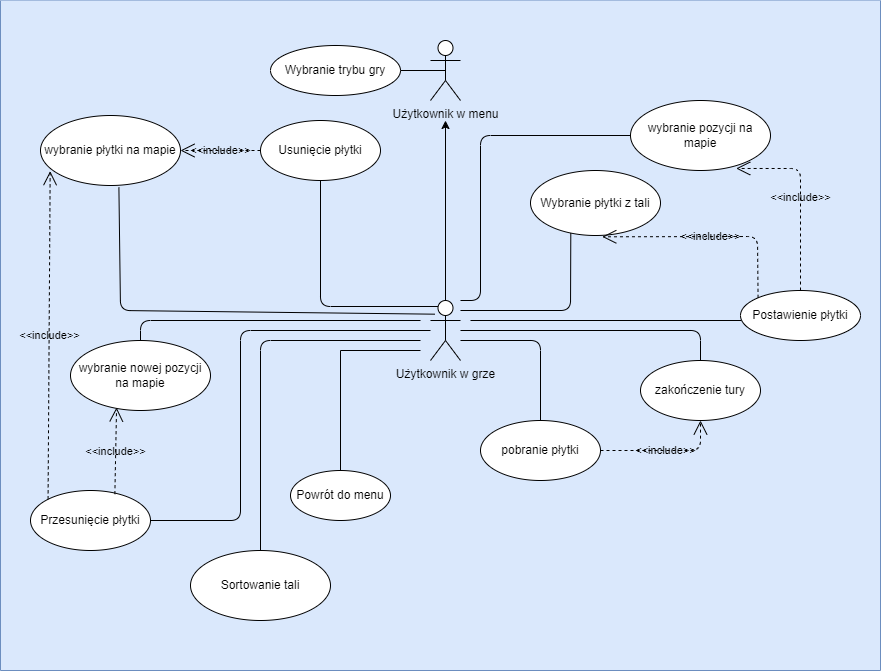
\includegraphics[width=\textwidth]{photos/use_case.png}
		\caption{Diagram przypadków użycia}
		\label{fig:usecase}
	\end{figure}
	
	% TODO
	\chapter{Specyfikacja zewnętrzna}% do akceptacji
	\label{ch:04}
	
	\section{Wymagania sprzętowe i programowe}
	Minimalne wymagania zostały opisane w dokumentacji Unity \cite{bib:wymagania_dokumentacja}, użytkownik powinien posiadać komputer z tymi bądź lepszymi komponentami:
		\begin{itemize}
			\item Windows 10 and Windows 11 tylko w wersji 64-bitowej
			\item CPU x64 z obsługą zestawu instrukcji SSE2.
			\item GPU kompatybilne z DX10, DX11 i DX12.
		\end{itemize}
		
		System był testowany na komputerze z komponentami:
		\begin{itemize}
			\item AMD Ryzen 9 7940HS w/ Radeon 780M Graphics 4.00 GHz
			\item 16,0 GB pamięci RAM
			\item System 64-bitowy Windows 11 
			\item NVIDIA GeForce RTX 4050
		\end{itemize}
	\section{Instalacja}
	Aby uruchomić grę w trybie edycyjnym, należy zainstalować poniższe oprogramowanie i biblioteki:
	\subsection{Unity}
	Do uruchomienia projektu wymagana jest instalacja Unity w wersji co najmniej 2022.3 . Więcej informacji, na temat instalacji, znajduje się \cite{bib:Unity_instalacja}. Aby pobrać i zainstalować Unity, należy:
	\begin{enumerate}
		\item Pobierz Unity Hub z oficjalnej strony: \url{https://unity.com/download}.
		\item Zainstaluj Unity Hub i dodaj wersję edytora Unity 2022.3 lub nowszą.
		\item Skonfiguruj środowisko projektu, upewniając się, że zainstalowane są wybrane moduły.
	\end{enumerate}
	\subsection{Python}
	Konieczne jest zainstalowanie Pythona w wersji 3.8 bądź nowsza, więcej informacji można znaleźć \cite{bib:link_do_instrukcji_python}.
	\begin{enumerate}
		\item Należy pobrać instalator z odpowiednią wersją oficjalnej strony 
		\url{https://www.python.org/downloads/}.
		\item Uruchomić instalacje.
	\end{enumerate}
	\subsection{Biblioteka ml-agents}
	Biblioteka ML-Agents Toolkit jest wymagana do wdrożenia komponentów sztucznej inteligencji w grze. Szczegółowa instrukcja instalacji znajduje się \cite{bib:link_do_instrukcji_ml-agents}. Konieczne jest zainstalowanie jej w środowisku Python jak i w Unity.
	\begin{enumerate}
	\item Przejdź do zakładki Okno (Window) w Unity 
	\item Wybierz Menedżer Pakietów (Package Manager)
	\item W okienko wyszukiwania wpisz \textit{ml-agents}
	\item Zainstaluj wybraną wersję
	\item W plikach projektu stwórz środowisko wirtualne Python przy użyciu \textit{Wiersza poleceń}
	\begin{verbatim}
		python -m venv nazwa_folderu
	\end{verbatim}
	bądź 
	\begin{verbatim}
		py -m venv nazwa_folderu
	\end{verbatim}
	
	\item Aktywuj środowisko przy użyciu:
	\begin{verbatim}
		nazwa_folderu\Scripts\activate
	\end{verbatim}
	
	\item Zainstaluj w środowisku wirtualnym potrzebne biblioteki
		\begin{verbatim}
		py -m pip install --upgrade pip
		pip install torch
		\end{verbatim}
		aby zainstalować konkretną wersję biblioteki pytorch, należy wpisać komendę:
		\begin{verbatim}
			pip install torch==(wybrana wersja)
		\end{verbatim}
		Ostatecznie należy wpisać komendę:
		\begin{verbatim}
			pip install mlagents
		\end{verbatim}
		Jeśli ta komenda wywoła błąd, należy wpisać:
		\begin{verbatim}
			pip install mlagents --use-feature=2020-resolver
		\end{verbatim}
		Aby zweryfikować, czy biblioteka została poprawnie zainstalowana, należy wpisać:
		\begin{verbatim}
			mlagents-learn --help
		\end{verbatim}
		Jeśli biblioteka jest poprawnie zainstalowana, to polecenie wyświetli dostępne komendy w ramach biblioteki ml-agents.
	\end{enumerate}
	
	\section{Aktywacja}
	Po poprawnej instalacji i konfiguracji bibliotek oraz oprogramowania, można uruchomić aplikacje.
	\\Aby włączyć symulacje aplikacji, należy wykonać następujące kroki:
		\begin{enumerate}
			\item Otwórz Unity Hub i wybierz projekt z listy w odpowiedniej wersji edytora Unity.
			\item Kliknij przycisk \texttt{Open}, aby załadować projekt.
			\item W edytorze Unity załaduj scenę \texttt{Menu}
			\item Naciśnij przycisk \textbf{Play}, aby uruchomić grę w trybie symulacji.
		\end{enumerate}
	Jeżeli gra została zbudowana jako aplikacja, aktywacja przebiega następująco:
		\begin{enumerate}
			\item Otwórz folder z plikami projektu (np. \texttt{Build/Release}).
			\item Uruchom plik wykonywalny (na Windows jest to plik typu \texttt{.exe}).
			
		\end{enumerate}
	Aby rozpocząć naukę sztucznej inteligencji (ML-Agents), należy wykonać kolejne polecenia:
		\begin{enumerate}
			\item Otwórz Unity Hub i wybierz projekt z listy w odpowiedniej wersji edytora Unity.
			\item Kliknij przycisk \texttt{Open}, aby załadować projekt.
			\item W edytorze Unity załaduj scenę \texttt{CP\_AI\_GAME}
			\item W \texttt{Wierszu poleceń} przejdź do plików gry
			\item Aktywuj środowisko wirtualne w Python
			\item Wpisz poniższą komendę:
				\begin{verbatim}
					mlagents-learn --run-id=nazwa
				\end{verbatim}
			\item Naciśnij przycisk \textbf{Play} w Unity.
		\end{enumerate}

	\section{Sposób obsługi}
	Sposób obsługi zawiera szczegółową instrukcję, jak korzystać z aplikacji z perspektywy użytkownika.
	\subsection{Zasady gry}
	
	Projekt gry Rummikub jest oparty na fizycznej grze planszowej, której zasady zostały opisane dokładnie w \cite{bib:rummikub_rules}.
	Gra wymaga od dwóch do czterech graczy. Gra podstawowa zawiera 106 płytek, w którym jest osiem serii o wartościach od jeden do trzynaście w czterech kolorach, oraz dwa jokery. Jokery to płytki specjalne, które mogą zastąpić każdą płytkę na mapie. Zadaniem każdego gracza jest jak najszybciej wyłożyć na stół wszystkie płytki, które zawiera w swojej tabliczce.
	W grze znajdują się dwa typy sekwencji płytek
		\begin{itemize}
			\item Grupy - jest to sekwencja płytek, w skład której wchodzą co najmniej trzy płytki o tej samej liczbie ale różnych kolorach. Joker może zastąpić płytkę w takiej sekwencji, grupa nie może zawierać więcej niż 4 płytki
			\item Serie - jest to sekwencja co najmniej trzech płytek w tym samym kolorze o różnych wartościach w kolejności od najmniejszej do największej. W takiej sekwencji może znajdować się maksymalnie 13 płytek, rozpoczynającą płytką jest zawsze o numerze jeden, a kończącą o numerze trzynaście.
		\end{itemize}
	Każdy gracz zaczyna rozgrywkę z czternastoma płytkami. Na początku rozgrywki gracze muszą wyłożyć sekwencje i grupy o łącznej wartości trzydziestu punktów i więcej. Każda płytka ma swoją wagę punktową, zależną od liczby wypisanej na płytce. Wartością wagową jokera jest liczba jaką zastępuje na planszy. 
	Dopóki gracz nie wykona pierwszego ruchu, nie może manipulować żadnymi płytkami na mapie. Gracz również nie może manipulować żadnymi sekwencjami na mapie w trakcie swojego pierwszego wyłożenia. Po zakończeniu pierwszej tury, gracz może wykładać grupy i serie oraz wykonywać akcje, takie jak:
		\begin{itemize}
			\item dokładanie płytek na końcu i początku sekwencji na mapie
			\item rozdzielać jedną większą sekwencje na dwie mniejsze
			\item podmieniać jokery na mapie z płytkami ze swojego stojaka.
			\item przebudowywać grupy na serie oraz serie na grupy  
		\end{itemize}
	Gracz musi w każdej turze wyłożyć co najmniej jedną płytkę, jeśli nie może tego zrobić, musi pobrać płytkę z banku, co kończy jego turę i uniemożliwia wykonanie ruchu na mapie.
	W grze obowiązuje limit czasu. Jeśli gracz nie zakończy swoich manipulacji przed upływem czasu, wszystkie jego ruchy należy cofnąć, a gracz dobiera płytkę z głównego banku.
	Gra może zakończyć się w dwóch momentach:
	\begin{enumerate}
		\item gdy jeden gracz wyłoży wszystkie płytki ze swojego stojaka
		\item jeśli w głównym banku skończą się płytki a gracz, który ma swoją turę, chce dobrać kolejną.
	\end{enumerate}
	Wynik gry zależy od płytek w stojaku gracza. Na końcu gry są podliczane wyniki na podstawie wag wartości płytek. Wagi jokerów są równe 30. Wygrywa ten, którego wynik jest najmniejszy.
	
	
	\subsection{Ekran aplikacji}
	Rozgrywka rozpoczyna się widokiem menu głównego gry
		\begin{figure}[H]
		\centering
		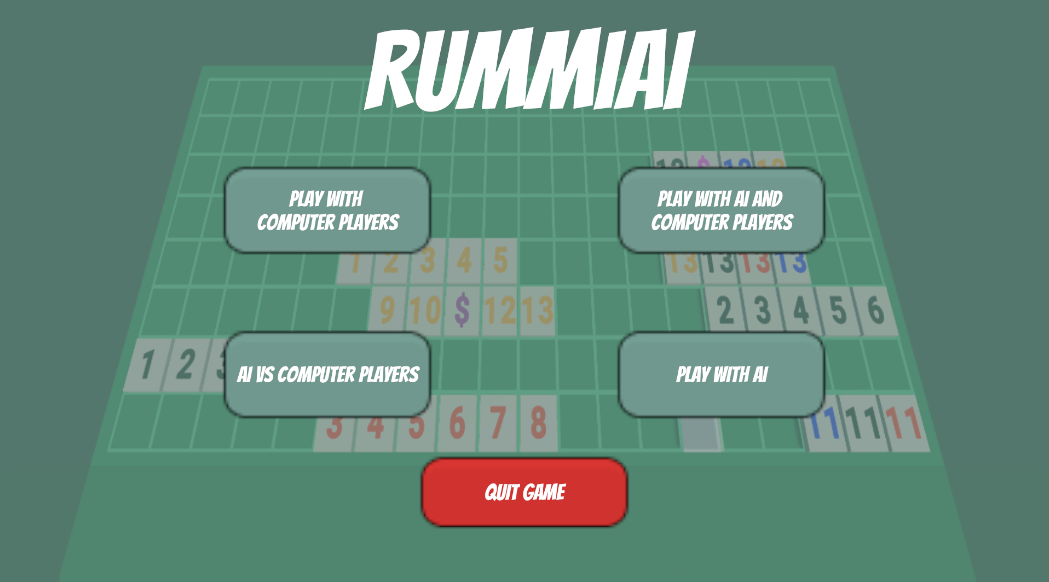
\includegraphics[width=\textwidth]{photos/Menu_gry.png}
		\caption{Menu gry}
		\label{fig:menugry}
		\end{figure}
		
		Na ekranie widać cztery przyciski, każdy z nich wykonuje co innego:
		\begin{itemize}
			\item \textbf{Play with computer players} - jest to rozgrywka, w której biorą udział trzej gracze komputerowi z predefiniowanymi ruchami wraz z użytkownikiem. Tryb służy jedynie do potencjalnego zapoznania się z grą i jej mechanikami.
			\item \textbf{Play with AI and computer players} - tryb gry, w którym użytkownik gra wraz z dwoma graczami komputerowymi oraz jednym graczem komputerowym z algorytmami sztucznej inteligencji. Jest to docelowy tryb projektu. 
			\item \textbf{AI vs computer players} - w tym trybie gry jest jeden gracz z algorytmami sztucznej inteligencji oraz trzej gracze komputerowi z predefiniowanymi ruchami. Ten tryb służy tylko do nauki modelu.
			\item \textbf{Play with AI} - ten tryb gry jest grą jeden na jeden, gdzie użytkownik gra przeciwko komputerowemu graczowi z uczeniem maszynowym. Ten tryb służy do walidacji nauki danego modelu.
			\item \textbf{Quit game} - przycisk służący do opuszczenia gry.
		\end{itemize}
		\begin{figure}[H]
			\centering
			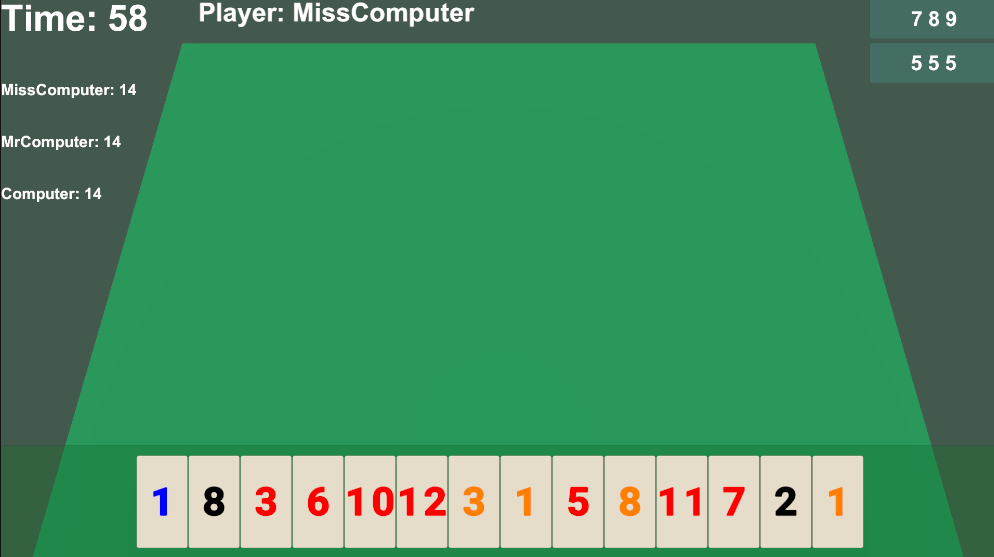
\includegraphics[width=\textwidth]{photos/start_gry.png}
			\caption{Przykładowy ekran początku gry}
			\label{fig:start_ekran_gry}
		\end{figure}
		Gra rozpoczyna się z każdym graczem posiadającym po czternaście płytek na swoim stojaku.\\Nad mapą widać napis:
		\begin{figure}[H]
			\centering
			
\includegraphics[width=\textwidth]{photos/current_player.png}
			\caption{Aktualna tura: Gracz X}
			\label{fig:napis_gracza}
		\end{figure}
		Napis ten informuje użytkownika, który gracz ma w danej chwili wykonuje turę ruchu. W tym miejscu mogą pojawić się różne napisy:
		\begin{itemize}
			\item Computer, MissComputer, MrComputer - są to wyznaczniki, że daną turę wykonuje gracz komputerowy o predefiniowanych ruchach.
			\item You - informacja, że to użytkownik może wykonać ruch.
			\item Agent - oznacza to, że gracz komputerowy z algorytmem uczenia maszynowego ma turę w danym momencie.
		\end{itemize}
				\begin{figure}[H]
			\centering
			
\includegraphics[width=\textwidth]{photos/time.png}
			\caption{widok czasu gry}
			\label{fig:czas}
		\end{figure}
		Na obrazku znajduje się reprezentacja czasu gry w aplikacji. Każda tura trwa pewną ilość czasu, jeśli dany gracz nie zakończy swojej tury przed czasem, wszystkie jego ruchy zostają cofnięte, oraz dostaje nową płytkę z banku. Jedna tura zazwyczaj trwa 60 sekund.
		\\Z lewej strony ekranu znajdują się pewne napisy. Są one reprezentacją listy gracz w danym trybie gry. Dostarcza również informacje, ile który gracz ma płytek na swoim stojaku. Lista graczy różni się w zależności od trybu gry:
				
		\begin{figure}[H]
		\centering
		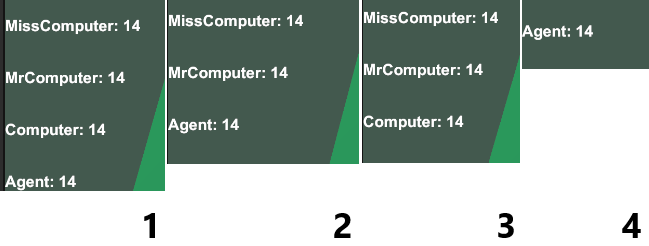
\includegraphics[width=\textwidth]{photos/lista graczy.png}
		\caption{widok listy graczy}
		\label{fig:lista_graczy}
		\end{figure}
		\begin{enumerate}
			\item Jest to lista graczy w trybie nauki. Znajdują się tutaj trzej gracze komputerowi z predefiniowanymi ruchami oraz jeden agent. Lista w tym trybie jest jedynie poglądowa dla użytkownika.
			\item To lista graczy z trybu gry użytkownik przeciwko dwóm graczom komputerowym z predefiniowanymi ruchami oraz jednemu graczowi komputerowemu z algorytmami uczenia maszynowego.
			\item Jest to lista z trybu gracz przeciwko trzem graczom komputerowym z predefiniowanymi ruchami.
			\item Ta lista jest z trybu gry użytkownik przeciwko gracz komputerowy z algorytmem uczenia maszynowego.
			
		\end{enumerate}
		Użytkownik ma możliwość interakcji z płytkami w stojaku.
		\begin{figure}[H]
			\centering
			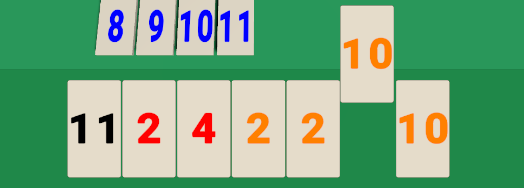
\includegraphics[width=\textwidth]{photos/dragable.png}
			\caption{widok stojaku z płytkami}
			\label{fig:przesuwanie}
		\end{figure}
		Przytrzymanie wybranej płytki pozwala na jej przesuwanie w prawo bądź lewo w celu ułożenia jej w konkretnej sekwencji.
		\\W prawym górnym rogu znajdują się przyciski, w zależności od momentu rozgrywki, są one różne:
		\begin{figure}[H]
			\centering
			
\includegraphics[width=\textwidth]{photos/out_turn_przyciski.png}
			\caption{przyciski poza turą}
			\label{fig:przyciski_poza_tura}
		\end{figure}
		Tak wygląda widok przycisków, gdy nie ma tury użytkownika : 
		\begin{itemize}
			\item pierwszy przycisk służy do sortowania względem serii.
			\item drugi przycisk służy do sortowania względem grup.
		\end{itemize}
		\begin{figure}[H]
			\centering
			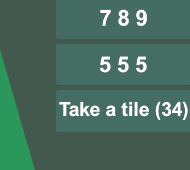
\includegraphics[width=\textwidth]{photos/przed_ruchem_przyciski.png}
			\caption{przyciski przed wykonaniem ruchu}
			\label{fig:przyciski_przed_ruchem}
		\end{figure}
		\FloatBarrier
		
		Tak wyglądają przyciski, gdy użytkownik ma swoją turę, ale jeszcze nie wykonał ruchu. Przycisk \texttt{Take a tile (34)} pozwala graczowi na pobranie płytki, wraz z czym kończy turę. Liczba w nawiasach na zdjęciu informuje, ile zostało płytek w głównym banku. Jeśli został użyty po wykonaniu ruchu na mapie, wszystkie manipulacje zostaną cofnięte. 
		\newpage
	\begin{figure}[H]
		\centering
		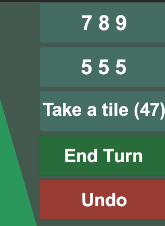
\includegraphics[width=0.7\textwidth]{photos/po_ruchu_przyciski.png}
		\caption{przyciski po wykonaniu ruchu}
		\label{fig:przyciski_po_ruchu}
	\end{figure}
	Przycisk \texttt{End Turn} wykona sprawdzenie, czy wszystkie sekwencje na mapie zawierają co najmniej trzy płytki. Jeśli funkcja wykryje błąd, tura nie zakończy się oraz zostanie pokazany komunikat o niepoprawnym zakończeniu tury.
	\\Przycisk \texttt{Undo} cofa wszystkie zmiany i wyłożenia, jakie użytkownik wykonał w trakcie danej tury.
	\newpage
	Jeśli gracz spróbuje zakończyć turę przyciskiem \texttt{End Turn}, podczas gdy na mapie co najmniej jedna sekwencja nie zawiera minimalnie trzech płytek, na ekranie użytkownika wyświetli się ten komunikat:
		\begin{figure}[H]
			\centering
			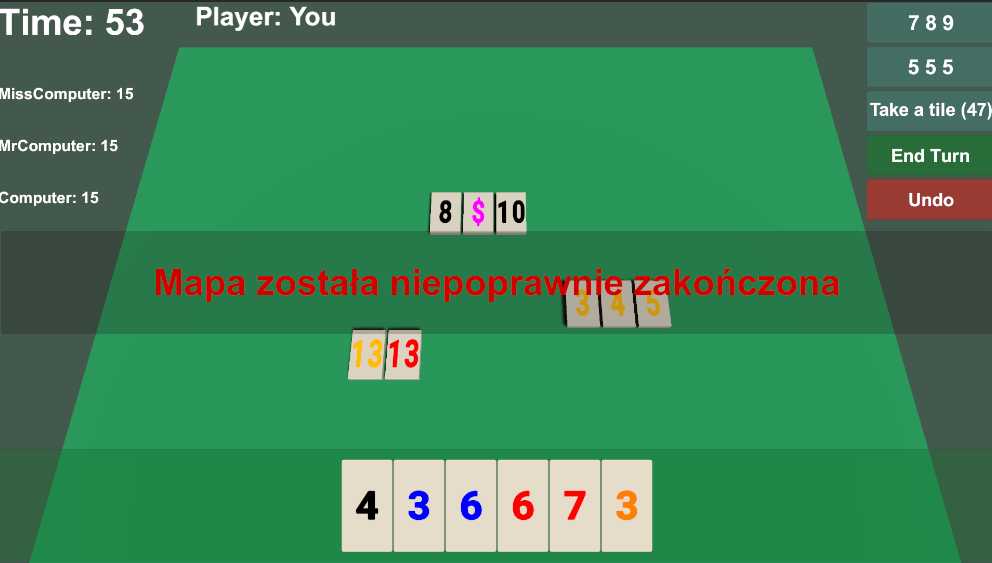
\includegraphics[width=\textwidth]{photos/zla_mapa.png}
			\caption{komunikat o źle zakończonej mapie}
			\label{fig:komunikat_zla_mapa}
		\end{figure}
		
	Jeśli gracz wykonuje swoją pierwszą turę, ale suma sekwencji, jakie wyłożył, nie jest równa bądź większa trzydzieści, to na ekranie pokaże się komunikat:
	\begin{figure}[H]
		\centering
		
\includegraphics[width=\textwidth]{photos/zla_pierwsza_tura.png}
		\caption{komunikat o źle zakończonej pierwszej turze}
		\label{fig:nie_ma_sumy_30}
	\end{figure}
	Gdy gracz już zakończył swoją pierwszą turę i w trakcie kolejnej tury wykona manipulacje sekwencjami na mapie nie wykładając przy tym ani jednej płytki ze swojego stojaka, pokaże się taki komunikat na mapie:
		\begin{figure}[H]
		\centering
		
\includegraphics[width=\textwidth]{photos/co_najmniej.png}
		\caption{komunikat braku wyłożonej płytki}
		\label{fig:nie_wylozona_plytka}
	\end{figure}
	Nie dozwolone jest, na daną turę, manipulowanie mapą bez wyłożenia nowej płytki.
	\\Jeżeli gracz zdecyduje się zabrać z planszy płytkę, która została położona przez niego bądź kogoś innego w innej turze, pojawi się na ekranie komunikat:
	\begin{figure}[H]
		\centering
		
\includegraphics[width=\textwidth]{photos/juz_polozone.png}
		\caption{komunikat przy niedozwolonym usuwaniu płytki}
		\label{fig:już_wylozona_plytka}
	\end{figure}
	Gdy pierwszy gracz wyłoży wszystkie płytki na mapę, pokaże się ekran zakończenia gry:
	\begin{figure}[H]
		\centering
		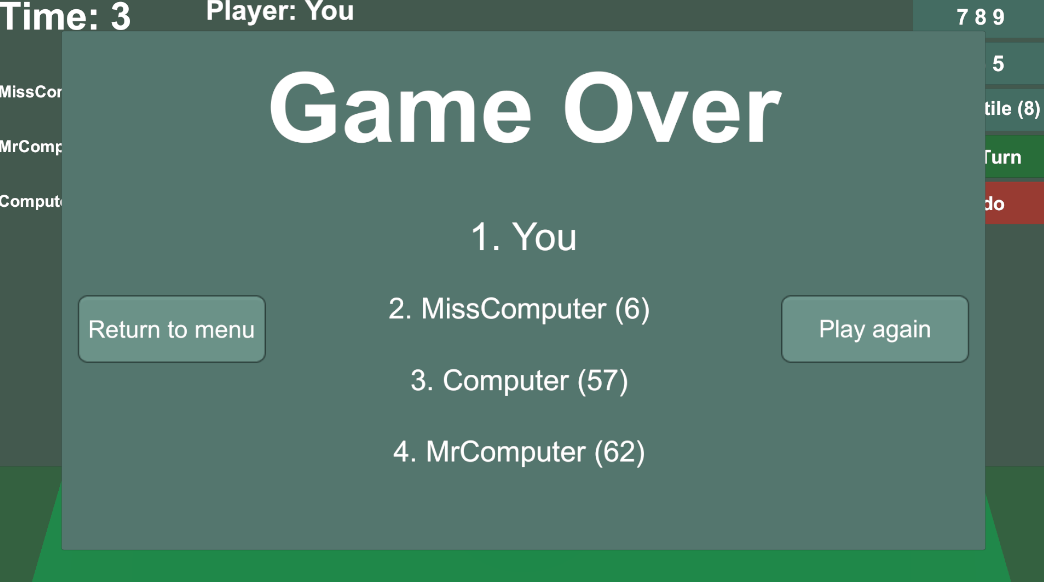
\includegraphics[width=\textwidth]{photos/endgame_screen.png}
		\caption{ekran końca gry}
		\label{fig:endgame_screen}
	\end{figure}
	Na zdjęciu widać hierarchię graczy w zależności od ich wyniku. Każdy gracz w hierarchii, pod zwycięzcą, ma w nawiasie zapisany wynik sumy płytek, które miał na swoim stojaku pod koniec gry. W takiej sytuacji wygrywa gracz, który nie ma już żadnych płytek na stojaku.
	\\Jeśli gra jednak zakończy się brakiem płytek w głównym banku, ekran końca gry będzie wyglądać tak:
	  	\begin{figure}[H]
	  	\centering
	  	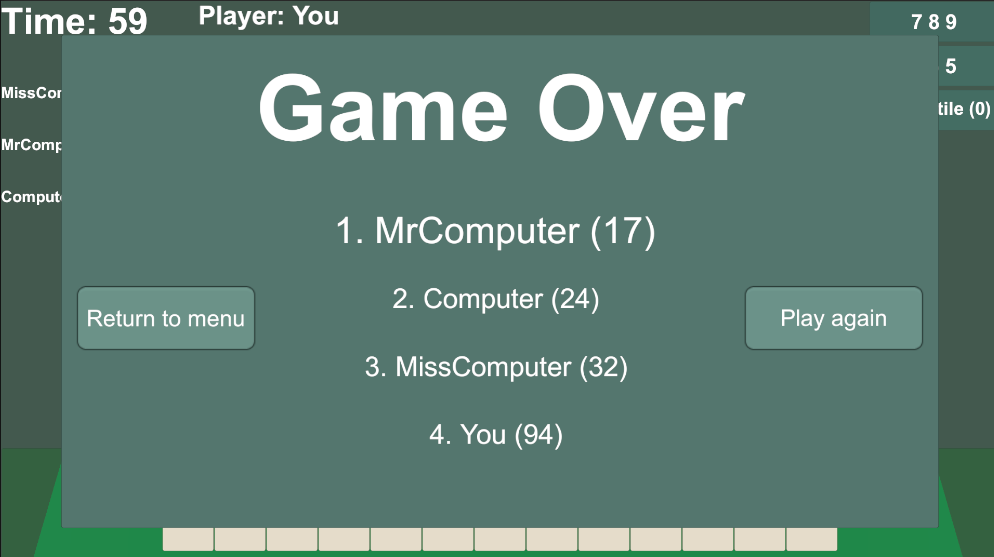
\includegraphics[width=\textwidth]{photos/endgame_pusty_bank.png}
	  	\caption{ekran końca gry przy pustym banku}
	  	\label{fig:endgame_screen_empty_bank}
	  \end{figure}
	  W takiej sytuacji, każdy gracz ma wyliczoną sumę płytek na swoim stojaku. W takiej sytuacji wygrywa gracz, którego suma punktów jest najmniejsza.
	  
	  Na ekranie końca gry, oprócz hierarchii, znajdują się dwa przyciski:
	  \begin{itemize}
	  	\item \textbf{Return to menu} - jego użycie przeniesie użytkownika do menu głównego gry.
	  	\item \textbf{Play again} - wykorzystanie tego przycisku pozwoli graczowi wzięcie udziału w nowej rozgrywce w tym samym trybie.
	  \end{itemize}
	  
	  Każda płytka w grze odpowiada obiektom wykorzystywanym w oryginalnej grze planszowej, oprócz płytek jokerów. Jokery w tej aplikacji wyglądają tak:
	  \begin{figure}[H]
	  	\centering
	  	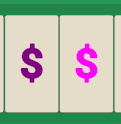
\includegraphics[width=0.4\textwidth]{photos/Jokery.png}
	  	\caption{jokery}
	  	\label{fig:jokery}
	  \end{figure}
	   W trakcie gry można również ją zatrzymać, jeśli użytkownik musi na chwilę odejść od urządzenia, albo jakby chciał zmienić tryb bez przymusu czekania na zakończenie rozgrywki. W tym przypadku może nacisnąć przycisk \texttt{Esc} aby uruchomił się ekran:
	  \begin{figure}[H]
	  	\centering
	  	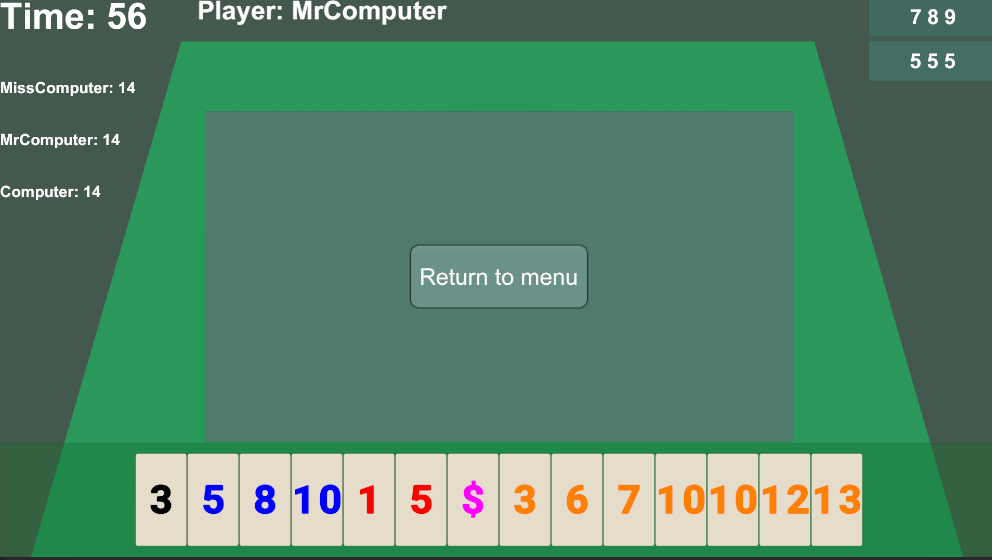
\includegraphics[width=0.8\textwidth]{photos/stop_game.png}
	  	\caption{Ekran zatrzymania gry}
	  	\label{fig:stop_game}
	  \end{figure}
	  W tym stanie, gra zostaje zatrzymana. Wciśnięcie przycisku \texttt{Return to menu} będzie skutkowało przedwczesnym zakończeniem gry i powrotem do menu głównego. Aby wznowić grę, użytkownik musi ponownie wcisnąć klawisz \texttt{Esc}.
	\subsection{Rozgrywka}
	Po wybraniu trybu gry, użytkownik widzi mapę rozgrywki. Zadaniem gracza jest, aby jak najszybciej wyłożyć płytki ze swojego stojaka.
	Podczas interakcji z mapą, pojawia się siatka, aby gracz wiedział, gdzie może płytka może być położona.
	Aby położyć płytkę na mapie, należy nacisnąć lewym przyciskiem myszy wybraną płytkę, a następnie przesunąć kursor myszy w stronę wybranej pozycji na mapie.
	\begin{figure}[H]
		\centering
		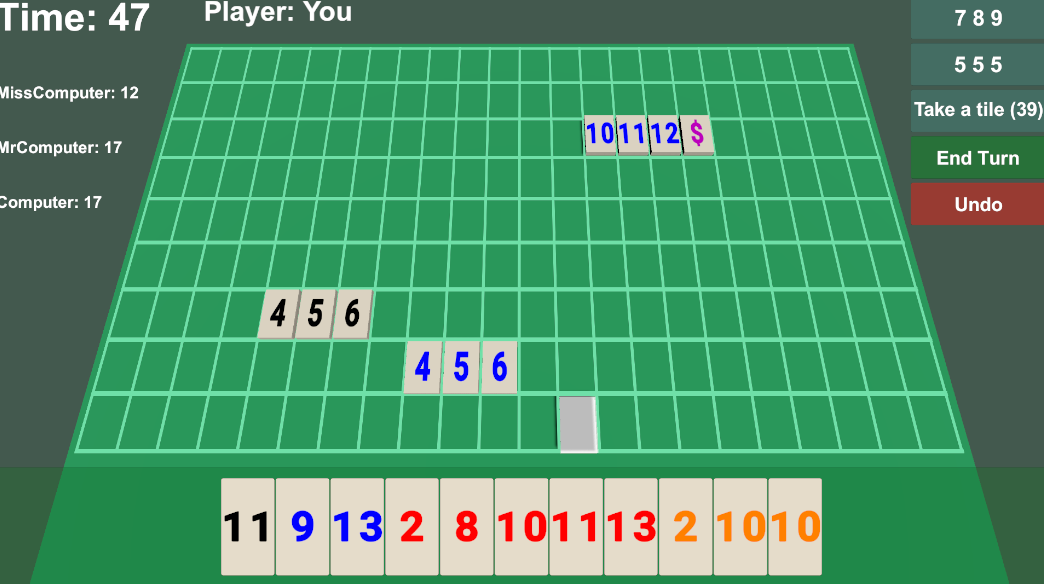
\includegraphics[width=\textwidth]{photos/w_turze.png}
		\caption{Kładzenie płytki na mapę}
		\label{fig:w_turze}
	\end{figure}
	Na ekranie widać obiekt, podobny do płytki. Gracz dzięki temu widzi, gdzie płytka będzie położona. Aby zakończyć akcję, wystarczy nacisnąć lewym przyciskiem myszy punkt na mapie. Jeśli gracz przeciągnie kursorem myszy na pole, na którym nie może położyć płytki, obiekt zostanie pokazany na czerwono
	\begin{figure}[H]
		\centering
		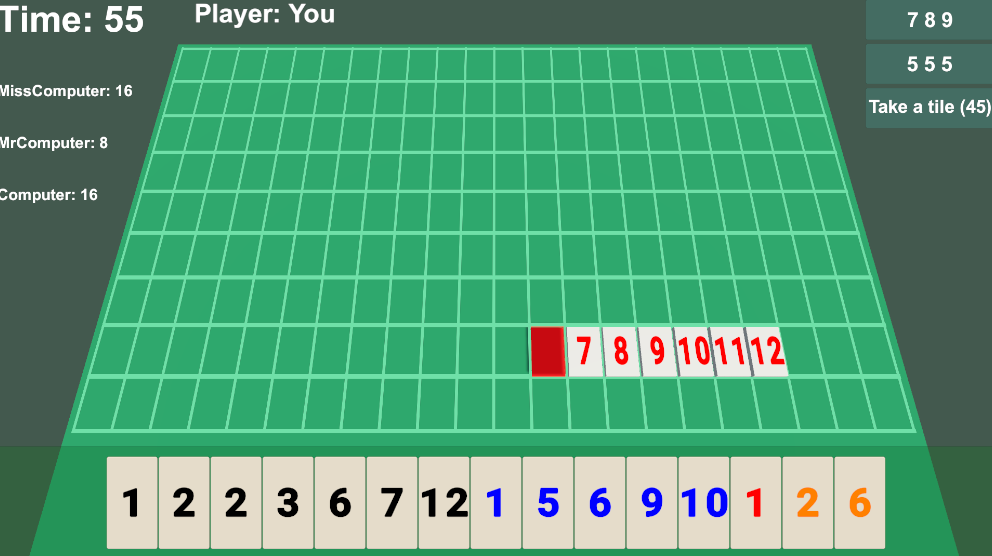
\includegraphics[width=\textwidth]{photos/zle_polozenie.png}
		\caption{Złe położenie płytki}
		\label{fig:zle_polozenie}
	\end{figure}
	Aby usunąć płytkę z mapy, należy wcisnąć klawisz \texttt{D}, a następnie kliknąć lewym przyciskiem myszy na płytkę, którą chce się usunąć. Ta akcja usuwa płytkę z mapy i przywraca ją do stojaka gracza. Użytkownik może usunąć jedynie płytki wyłożone w trakcie trwającej tury. Gracz, chcąc usunąć płytkę z mapy zobaczy czerwony obiekt jako kursor. Oznacza on, że nie można usunąć obiekt z miejsca, w którym obiektu nie ma. Obiekt zmienia kolor na biały, gdy zostanie umiejscowiony na pozycji, gdzie znajduje się płytka 
	\begin{figure}[H]
		\centering
		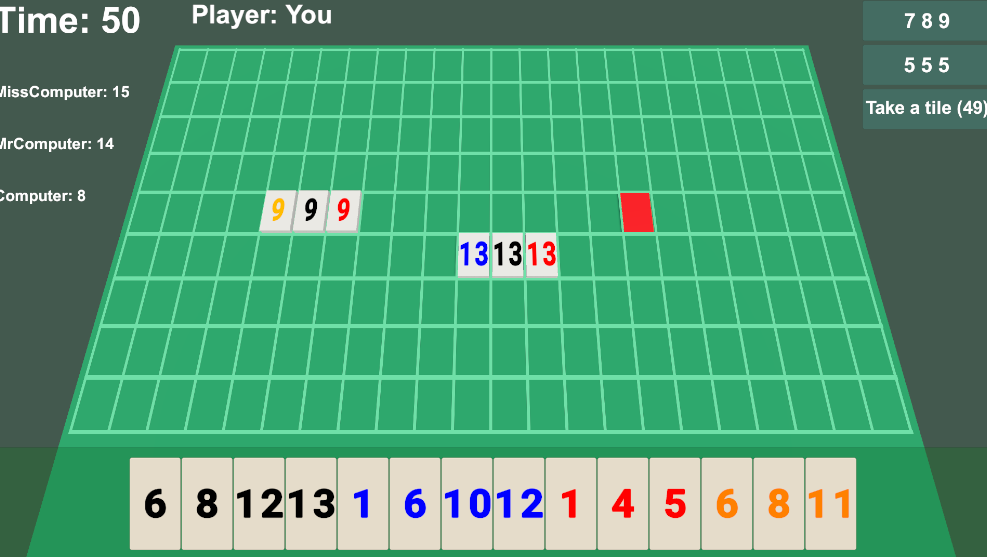
\includegraphics[width=\textwidth]{photos/usuwanie.png}
		\caption{wygląd usuwania płytki}
		\label{fig:usuwanie}
	\end{figure}
	Gdy gracz chce przesunąć płytkę na mapie, musi najpierw nacisnąć prawym przyciskiem myszy na wybraną płytkę. Następnie wybrać nową pozycję na mapie i nacisnąć lewy przycisk myszy na wybranej pozycji. W trakcie przesuwania płytki pojawia się obiekt tak samo, jak przy wykładaniu nowej płytki
	\\Jeśli gracz zdecyduje się zaprzestać wykonywania którejś akcji jak wykładania czy przesuwania, musi nacisnąć klawisz \texttt{Q}
	% TODO
	\chapter{Specyfikacja wewnętrzna}% TODO
	\label{ch:05}
	Specyfikacja wewnętrzna opisuje szczegóły techniczne implementacji projektu. Projekt został zrealizowany w środowisku Unity, jego kluczowe komponenty zostały zaimplementowane z C\#. To pozwoliło zaimplementować logikę gry, obiekty wykorzystywane w grze oraz gracza komputerowego z algorytmami uczenia maszynowego.
	\section{Biblioteka ML-Agents}
	Unity ML-Agents Toolkit to biblioteka służąca do implementowania i trenowania agentów z algorytmami uczenia maszynowego. Biblioteka pozwala na wykorzystanie metod takich jak uczenie ze wzmocnieniem, uczenie nadzorowane oraz uczenie w grupie. Biblioteka ML-Agents została wybrana do implementacji przeciwnika komputerowego w grze Rummikub, ponieważ:
	
	\begin{itemize}
		\item Umożliwia łatwe tworzenie środowiska treningowego w Unity.
		\item Pozwala dostosowywać metody modelu bezpośrednio do mechanik gry.
		\item Daje możliwość modyfikacji zmiennych modelu.
	\end{itemize}
	
	Kluczowymi komponentami ML-Agents są obserwacje, akcje oraz nagrody. 
	\begin{enumerate}
		\item Obserwacje dają agentowi potrzebne informacje, aby zaplanować swoje kolejne ruchy. Ilość obserwacji jest ustalana przy implementacji statycznie, nie ma możliwości zmieniać ilości obserwacji w trakcie rozgrywki.
		\item Akcje są funkcjami, jakie podejmuje na bazie obserwacji oraz nagród, jakie otrzymuje. Agent podejmuje akcje, dzielą się one na dwa typy
		\begin{itemize}
			\item akcje ciągłe - model wyznacza akcje z podanego przedziału liczbowego w wartościach zmiennoprzecinkowych, zazwyczaj od -1 do 1. Takie akcje są najlepsze przy funkcjach ruchu czy rotacji.
			\item akcje dyskretne - akcje modelu z podanego przedziału liczbowego w wartościach całkowitych. Najlepsze do konkretnych decyzji, jak wybieranie indeksów płytek w liście.
		\end{itemize}
		\item Otrzymywanie nagród i kar za konkretne działania dają agentowi informacje, jakie ruchy powinien wykonywać a jakie nie.
	\end{enumerate}
	Decyzje agenta są interpretowane jako wartości liczbowe, przy implementacji należy przypisać konkretnych wartościom funkcje. W zależności od decyzji agenta, należy mu przypisać nagrodę bądź karę. Z czasem agent uczy się, jakie decyzje są najbardziej opłacalne i częściej je wykonuje.
	
	Zmienne modelu mogą być modyfikowane w plikach typu \texttt{.yaml}. Na stronie \cite{bib:parametry_yaml} jest to dokładniej opisane.
	\begin{figure}[H]
		\centering
	\begin{lstlisting}
		behaviors:
			behaviors_name:
				trainer_type: ppo
				hyperparameters:
					batch_size: 10
					buffer_size: 100
					learning_rate: 3.0e-4
					beta: 5.0e-4
					epsilon: 0.2
					lambd: 0.99
					num_epoch: 3
					learning_rate_schedule: linear
					beta_schedule: constant
					epsilon_schedule: linear
				network_settings:
					normalize: false
					hidden_units: 128
					num_layers: 2
				reward_signals:
					extrinsic:
						gamma: 0.99
						strength: 1.0
				max_steps: 500000
				time_horizon: 64
				summary_freq: 10000
	\end{lstlisting}
	\caption{Przykładowe środowisko .yaml .}
	\label{fig:model_ml-agents:listings}
	\end{figure}
	Modyfikacja parametrów środowiska pozwala na dostosowanie modelu do aplikacji, w której jest implementowanie.
	
	Każdy parametr odpowiada innej funkcjonalności modelu:
	\begin{itemize}
		\item \textbf{behaviors} - jest główną sekcją definiującą zachowanie agenta. Zawiera wszystkie szczegóły dotyczące jego treningu.
		\item \textbf{behaviors\_name} - nazwa konkretnego zachowania, musi być identyczna do zaimplementowanej nazwy w Unity.
		\item \textbf{trainer\_type} - Typ algorytmu używanego do treningu. W przykładzie zawarty jest algorytm ppo (Proximal Policy Optimization).
		\item \textbf{hyperparameters} - przedział zmiennych algorytmu:
		\begin{enumerate}
			\item batch\_size - liczba próbek przetwarzanych w jednej iteracji.
			\item buffer\_size - liczba przechowywanych danych w pamięci bufora przez aktualizacją sieci.
			\item learning\_rate - określone tempo aktualizacji wag modelu podczas każdej iteracji.
			\item beta - współczynnik entropii, im wyższa wartość, tym model jest bardziej skłonny do eksploracji nowych strategii podczas nauki.
			\item epsilon - wyznacza maksymalną wartość, z jaką może zmieniać się polityka (policy) w jednej aktualizacji.
			\item lambd - współczynnik wygaśnięcia, do balansowania między dokładnością a stabilnością wyceny nagrody.
			\item num\_epoch - liczna iteracji gradientowych dla każdej próbki.
			\item learning\_rate\_schedule, beta\_schedule, epsilon\_schedule - określają jak wartości zmiennych \texttt{learning\_rate}, \texttt{beta} oraz \texttt{epsilon} zmieniają się w czasie treningu.
		\end{enumerate}
		\item \textbf{network\_settings} - definiuje strukturę sieci neuronalnej, której używa agent:
			\begin{enumerate}
				\item normalize - definiuje, czy dane wejściowe mają zostać zoptymalizowane czy nie.
				\item hidden\_units - liczba jednostek w każdej warstwie ukrytej sieci neuronalnej.
				\item num\_layers - ilość warstw sieci neuronalnej.
			\end{enumerate}
		\item \textbf{reward\_signals} - definiuje sygnał nagrody dla agenta. Tutaj jest użyty typ \texttt{extrinsic}, czyli nagroda bazująca na środowisku:
			\begin{enumerate}
				\item gamma - współczynnik wygaśnięcia, który określa w jakim stopniu agent bierze pod uwagę przyszłe nagrody.
				\item strength - skala wpływu sygnału na trening.
			\end{enumerate}
		\item \textbf{max\_steps} - Maksymalna liczba kroków treningowych, jakie może wykonać agent. Po osiągnięciu tej wartości, model nie może być dalej uczony.
		\item \textbf{time\_horizon} - maksymalny czas, po jakim agent kończy zbieranie danych do bufora.
		\item \textbf{summary\_freq} - określa, co ile zostają wygenerowane dane podsumowania treningu.
	\end{itemize}
	 
	\section{Klasa PlayerIA}
	\section{Klasa Tile}
	\section{Mechanika gry}
	\section{Struktura danych}
	
	% TODO
	\chapter{Weryfikacja i walidacja}% TODO
	\label{ch:06}
	
	\section{Testowanie}
	\section{Wykryte błędy}
	
	
	
	% TODO
	\chapter{Podsumowanie i wnioski}% TODO
	
	\section{Napotkane problemy}%TODO
	\section{Możliwy rozwój}%TODO
	
	
	
	\backmatter
	
	%\bibliographystyle{plplain}  % bibtex
	%\bibliography{biblio} % bibtex
	\printbibliography           % biblatex
	\addcontentsline{toc}{chapter}{Bibliografia}
	
	\begin{appendices}
		
		% TODO
		\chapter{Spis skrótów i symboli}
	
		
		% TODO
		\chapter{Źródła}
		
		
		% TODO
		\chapter{Lista dodatkowych plików, uzupełniających tekst pracy} 
		
		
		\listoffigures
		\addcontentsline{toc}{chapter}{Spis rysunków}
		\listoftables
		\addcontentsline{toc}{chapter}{Spis tabel}
		
	\end{appendices}
	
\end{document}


%% Finis coronat opus.

